\begin{song}{title=\predtitle\centering Nagasaki Hirošima \\\large Mňága \&  Žďorp  \vspace*{-0.3cm}}  %% sem se napíše jméno songu a autor
\begin{centerjustified}
\nejnejvetsi

\sloka
	^{A\z }Tramvají ^{E\z }dvojkou ^{D\z }jezdíval ^{E}jsem do ^*{\z A}Žideni c, ^{E\,\,D\,\,E}

	z ^{A}tak velký ^{E\z }lásky ^{D\z}většinou ^{E\z }nezbyde ^{F#mi\z }nic.~~~

	Z ^{D\z }takový ^{A\z}lásky ^{D\z}jsou kruhy ^{A\z}pod ^{\z E}očima

	a dvě ^*{A}sp álený ^{E\z }srdce -- ^{D\z }Nagasaki ^{E\z}Hirošima. ^{A\,\,E\,\,D\,\,E}

\sloka
	Jsou jistý věci, co bych tesal do kamene,
	
	tam, kde je láska, tam je všechno dovolené
	
	a tam, kde není, tam mě to nezajímá.
	
	Jó dvě spálený srdce Nagasaki Hirošima.

\sloka
	Já nejsem svatej, ani ty nejsi svatá,
	
	jablka z ráje bejvala jedovatá,
	
	jenže hezky jsi hřála, když mi někdy byla zima.
	
	Jó dvě spálený srdce Nagasaki Hirošima.

\sloka
	Tramvají dvojkou jezdíval jsem do Židenic,
	
	z takový lásky většinou nezbyde nic.
	
	Z takový lásky jsou kruhy pod očima

	/: a dvě spálený srdce Nagasaki Hirošma. :/
	
	/: A dvě spálený srdce Nagasaki Hirošma. :/

\end{centerjustified}
\setcounter{Slokočet}{0}
\end{song}


\begin{figure}[h]
\predtitle\centering
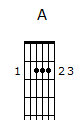
\includegraphics[width=3cm]{../Akordy/a.png}
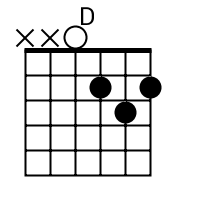
\includegraphics[width=3cm]{../Akordy/d.png}
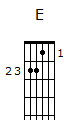
\includegraphics[width=3cm]{../Akordy/e.png}
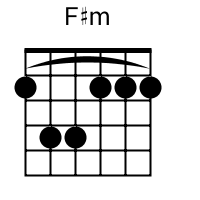
\includegraphics[width=3cm]{../Akordy/fxm.png}
\end{figure}
